% !TeX root = report.tex
\documentclass[uplatex,dvipdfmx,a4paper,11pt,jafont=haranoaji]{bxjsarticle}

\setpagelayout+{top=18mm,bottom=18mm,left=20mm,right=20mm,includeheadfoot=false,headsep=6mm}
\usepackage{amsmath,amssymb}
\usepackage{bm}
\usepackage{booktabs}
\usepackage{graphicx}
\usepackage{placeins}
\usepackage{float}
\usepackage{capt-of}
\usepackage{needspace}
\usepackage{enumitem}
\setlist{itemsep=1pt,topsep=3pt,parsep=0pt}
\makeatletter
\patchcmd{\subsection}{\Cvs \@plus.5\Cdp \@minus.2\Cdp}{.65\Cvs \@plus.3\Cdp \@minus.1\Cdp}{}{}
\patchcmd{\subsection}{.5\Cvs \@plus.3\Cdp}{.25\Cvs \@plus.2\Cdp}{}{}
\makeatother
\renewcommand{\arraystretch}{1.12}
\AtBeginEnvironment{table}{\small}
\setlength{\textfloatsep}{12pt plus 2pt minus 2pt}
\setlength{\floatsep}{10pt plus 2pt minus 2pt}
\newcommand{\answerpart}[1]{\par\Needspace{6\baselineskip}\subsection*{#1}}
\pretocmd{\section}{\Needspace{10\baselineskip}}{}{}
\usepackage{fancyhdr}
\setlength{\headheight}{16pt}
\usepackage[dvipdfmx]{hyperref}
\usepackage{pxjahyper}
\hypersetup{hidelinks}
\urlstyle{same}

\newcommand{\assignment}{最適化 レポート課題}
\pagestyle{fancy}
\fancyhf{}
\fancyhead[R]{\assignment}
\fancyfoot[C]{\thepage}
\renewcommand{\headrulewidth}{0pt}
\fancypagestyle{plain}{%
  \fancyhf{}%
  \fancyhead[R]{\assignment}%
  \fancyfoot[C]{\thepage}%
  \renewcommand{\headrulewidth}{0pt}%
}
\newcommand{\norm}[1]{\lVert #1\rVert_2}

\begin{document}

\title{移動充電車両に支援されるUAVの非線形軌道最適化モデルの検討}
\author{計数工学科 03260626 齋藤晴輝}
\date{2026年11月20日}
\maketitle
\thispagestyle{fancy}

対象は Yuan ら\cite{yuan}の論文（以下、原論文）である。式番号 (1)〜(27) は原論文の番号をそのまま使い、本レポートで新しく置く式は (R)、(C0)〜(C2) のように英字を付ける。
独自計算では原論文の物理係数（$v_d=36$ km/h、$v_c=10.8$ km/h、$\zeta=2.5$/h、$s_{\min}=30$ s など）を用いた。原論文の数値を引用する箇所と、独自計算の結果を区別して述べる。実装・入力・実験記録の保存先を文献\cite{repo}に示す。

%======================================================================
\section{問1：問題設定とモデル}

\answerpart{解きたい問題}
1機のUAVが、始点 $r^0$ から終点 $r^f$ まで飛ぶ間に $\tau$ 個のタスク地点 $a_1,\dots,a_\tau$（観測対象など）を全て訪れる。
電池が足りないので途中で充電するが、充電は地上の移動充電車両の上でしかできず、車両は地形の制約で $J$ 個の領域（数値例では円板 $\mathcal C_j=\{x:\norm{x-o_j}\le\rho_j\}$）の中しか走れない。
UAVが決めることは、タスクを訪れる順番、どこで・いつ・どれだけ充電するか（部分充電を含む）、および各区間の移動であり、目的は全ミッション時間の最小化である。
訪問順と充電の有無は離散的な選択なので、通常は整数変数を含む混合整数計画になり、タスク数が増えると計算時間が急増する。
原論文の主眼は、この離散選択を整数変数なしの滑らかな非線形計画（NLP）で近似することにある。

\answerpart{変数と目的関数}
軌道を $N$ 個の時点で表し、変数 (10) は次の4種類である。
\begin{itemize}
  \item $r_k\in\mathbb R^2$（$k\in[N]$）：時点 $k$ のUAVの位置。区間内は直線で移動すると考える。
  \item $e_k\in[0,1]$：時点 $k$ の電池残量（満充電を1とする割合）。
  \item $s_k>0$（$k\in[N-1]$）：時点 $k$ から $k+1$ までの区間の所要時間。
  \item $c_k\ge0$：その区間のうち車両上で充電する時間。$c_k=s_k$ なら「車両に載って充電」、$c_k=0$ なら「自力で飛んで放電」に対応する。
\end{itemize}
目的関数は総時間 $\sum_{k=1}^{N-1}s_k$ (1) で、移動時間と充電時間の和、すなわち任務の完了時刻である。

\answerpart{制約}
滑らかな制約 (11) は、端点 $r_1=r^0$、$r_N=r^f$、$e_1=e_{\max}$、UAVの速度上限 $\norm{r_{k+1}-r_k}\le v_ds_k$ (3)、電池と区間時間の上下限 $e_{\min}\le e_{k+1}\le e_{\max}$、$s_{\min}\le s_k\le s_{\max}$、および電池の統一ダイナミクス
\begin{equation*}
  e_{k+1}=f(e_k,s_k,c_k):=f_c(e_k,c_k)+f_d(e_k,s_k-c_k)-e_k \tag{6}
\end{equation*}
である。$f_c,f_d$ は時間 $t$ だけ充電・放電した後の残量で、$f_c(e,0)=f_d(e,0)=e$ (5) を仮定するので、$c_k=0$ なら放電、$c_k=s_k$ なら充電の式に一致する (7)。
数値例では放電を一定率 $f_d(e,t)=e-\zeta t$ (27)、充電を定電流・定電圧（CC--CV）方式とする (26)。初期残量 $e<e_{\mathrm{th}}$ なら $\theta=(e_{\mathrm{th}}-e)/\kappa$ までは $e+\kappa t$、以降は $e_{\max}-(e_{\max}-e_{\mathrm{th}})\exp(-(t-\theta)/\sigma)$ となる。$e\ge e_{\mathrm{th}}$ なら初めから $e_{\max}-(e_{\max}-e)\exp(-t/\sigma)$ を用い、$\sigma=(e_{\max}-e_{\mathrm{th}})/\kappa$ である。

離散的な選択は選言制約 (12) で表す。
\begin{equation*}
  \bigvee_{k\in[N]}\{r_k=a_i\}\ (i\in[\tau]),\qquad
  \bigvee_{j\in[J]}\left\{c_k=s_k,\ g_j(r_k,r_{k+1},s_k)\le0\right\}\vee\{c_k=0\}\ (k\in[N-1]). \tag{12}
\end{equation*}
前者は「各タスクをどこかの時点で訪れる」、後者は「各区間は放電か、どれかの領域 $j$ での充電のどちらか」を表す。
数値例の $g_j$ は
\begin{equation*}
  g_j(r_k,r_{k+1},s_k)=\bigl(\norm{r_k-o_j}-\rho_j,\ \norm{r_{k+1}-o_j}-\rho_j,\ \norm{r_{k+1}-r_k}-v_cs_k\bigr) \tag{24}
\end{equation*}
で、充電区間の両端が車両の走れる領域内にあり、その区間の移動が車両の最高速度 $v_c$ 以下であることを課す。
以上の (1)、(11)、(12) が原問題 (13) である。

\answerpart{提案手法の特徴}
\begin{enumerate}
  \item \textbf{最小値による書き換え}：(12) を「候補ごとの違反量の最小値が0」と書く (17)。
  例えばタスク $i$ では候補値 $z_k=\norm{(r_k-a_i,\varepsilon)}$ とし $\min_kz_k=\varepsilon$ を課す（$z_k=\varepsilon\iff r_k=a_i$）。
  充電の候補では不等式の違反を滑らかな関数 $\psi_\delta$ (18) で測り、$(c_k-s_k,\psi_\delta(g_j),\varepsilon)$ のノルムを候補値とする。
  \item \textbf{$\ell_p$ ノルムによる滑らかな最小値}：$\min_iz_i$ を $\phi_p(z)=(\sum_iz_i^{-p})^{-1/p}$ (19) で置き換え、全ての関数が微分可能なNLP (23) を得る。
  定理1は、最小値を取る候補が $m$ 個、最小値と次の値の差が $\Delta$ のとき、
  候補数を $n$ として $\exp\!\bigl(\frac{m-n}{pm(1+\Delta/z_{\min})^p}\bigr)z_{\min}\le m^{1/p}\phi_p(z)\le z_{\min}$ (21) と、勾配の方向についての同様の評価 (22) を与える。
  $p$ が大きく候補の差が大きいほど、値も勾配の方向も元の最小値に近づく。
  \item \textbf{ホモトピー法}：$\varepsilon$ が小さく $p$ が大きいと悪条件になるので、$\varepsilon_0=0.2$、$p_0=2$ から $\varepsilon\leftarrow\max(0.6\varepsilon,5\times10^{-4})$、$p\leftarrow\min(1.2p,12)$ と段階的に鋭くし、各段階のNLPを拡張ラグランジュ法（内側はL-BFGS）で解いて次の初期値にする（Algorithm 1）。
\end{enumerate}
数値実験では $\tau=1,\dots,9$ の各100例で、整数変数を使う定式化（MINLP、SCIP/Juniperで10時間打ち切り）と比べ、計算時間の中央値が1分未満で、目的値と制約違反は同程度だったと報告している（図3）。

\FloatBarrier
%======================================================================
\section{問2：良い点と問題点}

\answerpart{良い点}
\begin{description}[leftmargin=1em]
  \item[部分充電と非線形充電を一つの式で扱う] (6) は $c_k$ が $0$ か $s_k$ かで放電と充電を切り替え、(5) を満たす任意の写像を使える。満充電を前提にする多くの従来モデルより現実に近い。
  \item[整数変数を使わない] 訪問時点と充放電の選択を連続変数のNLPで探せるので、汎用の滑らかな最適化法が使え、計算時間が大きく減る（図3で中央値1分未満）。
  \item[近似の質を定量化している] 定理1で $\phi_p$ の値と勾配方向の誤差を評価し、数値実験でも (21)、(22) の指数項がほぼ1であることと、元の制約の違反量を報告している。
\end{description}

\answerpart{問題点1：サービス可能の仮定だけでは、1台運用の再訪を保証しない}
原論文は「各領域内で移動充電車両がUAVにサービスできる」と仮定し（II-C節）、車両の位置を変数 (10) に含めない。
本稿では、このサービスを各領域1台で実現する運用を考え、その適用限界を調べる。原論文が車両数や再配置を陽に規定していると解釈するものではない。
(24) は一つの充電区間の両端と、その区間内の移動しか見ていない。
しかし各領域の車両が1台なら、同じ領域で充電する区間 $a<b$ が連続するとき、車両は区間 $a$ の終点 $r_{a+1}$ から区間 $b$ の始点 $r_b$ まで、その間の時間で移動しなければならない。
時刻を $t_1=0$、$t_{k+1}=t_k+s_k$ とすると、少なくとも
\begin{equation*}
  \norm{r_b-r_{a+1}}\le v_c\,(t_b-t_{a+1})=v_c\sum_{k=a+1}^{b-1}s_k \tag{R}
\end{equation*}
が必要である（区間 $a$ の間、車両はUAVを載せているので、その時間は使えない）。原制約 (11)、(12) は (R) を含まない。

\textbf{反例}：半径2 kmの円板の中に $A=(-1,0)$、$B=(1,0)$ kmを置き、Aで30 s充電、AからBへ200 sで飛行、Bで30 s充電する。電池・速度・領域の原制約は全て満たすが、車両はAからBへの2 kmに $2/10.8$ h $=666.7$ s必要で、(R) を1.4 km破る。
待ち時間を足せばよいとも限らない。Aで充電した後に10 km離れたBで再び充電する例（両方の充電がないと電池が持たない配置）では、車両に3333 s必要だが、充電しない区間の長さは $e_{\max}-e_{\min}\ge\zeta\Delta t$ より $\Delta t\le0.4$ h $=1440$ s に制限されるので、待つだけでは直せない。

\textbf{さらに、モデルは車両が速さ $v_d$ で「跳ぶ」ことを許す}。
充電区間の移動は $v_c$ 以下に制限されるが、充電を一度切れば放電区間として $v_d$ で円板の中を移動し、同じ円板の別の点で再び充電できる。
車両の移動を省略したまま、接点を $v_d=3.3v_c$ 相当で移せることになる。本検討では、実際にこの形の解が多数現れた。
\begin{figure}[H]
  \begin{minipage}[c]{0.47\textwidth}
    \centering
    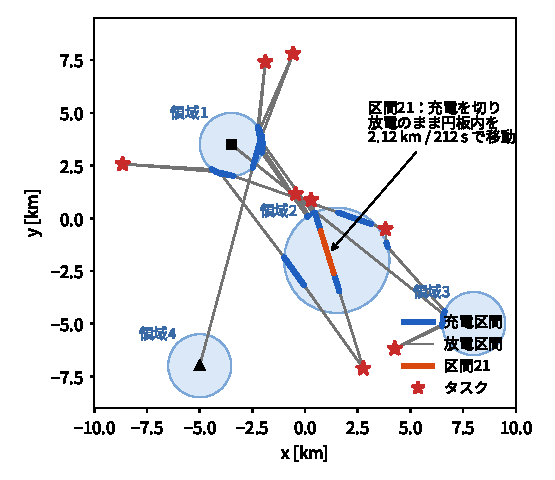
\includegraphics[width=\textwidth]{fig/fig-carrier.pdf}
    \caption{原制約を満たすが1台の車両では実行できない解の例（$\tau=8$）。区間20と22は同じ領域2での充電で、間の区間21は放電のまま円板内を2.12 km移動する。車両は212 sで0.64 kmしか動けない。区間・領域番号は1始まり。}
    \label{fig:carrier}
  \end{minipage}\hfill
  \begin{minipage}[c]{0.49\textwidth}
    \centering\small
    \captionof{table}{原制約を満たす解のうち、1台の車両が次の充電に間に合わない解の数}
    \label{tab:carrier}
    \begin{tabular}{@{}lrrr@{}}
      \toprule
      $\tau$ & 原制約を満たす & 再訪あり & 間に合わない \\
      \midrule
      1 & 100 & 34 & 10 \\
      3 & 99 & 81 & 50 \\
      5 & 100 & 97 & 70 \\
      7 & 99 & 99 & 85 \\
      9 & 99 & 99 & 96 \\
      \midrule
      1〜9計 & 894 & 755 & 590 \\
      \bottomrule
    \end{tabular}
  \end{minipage}
\end{figure}
再実装で得た、原制約を残差 $10^{-6}$ 以下で満たす解894個（$\tau=1,\dots,9$ の各約100例）に (R) を当てると、車両の初期位置を円板内で自由に選べるとしても、表\ref{tab:carrier}のとおり590個で車両が間に合わなかった。
同じ領域での連続充電は1訪問と数え、放電等を挟んで再開する場合を再訪とした。
不足距離の中央値は0.78 km、最大3.14 kmである。最も多い形（354個）が上の「跳び」で、図\ref{fig:carrier}はその例である。
一方、原論文の図1の解は、唯一の再訪で2.675 kmの移動に7.086 km分の時間があり (R) を満たす（図1・図2aの描画データから読み取った）。
したがって原論文の例が誤っているのではなく、\textbf{モデルが車両の運用可能性を保証しない}ことが問題である。
各領域1台の運用では、計画どおりに飛んでも充電地点に車両がいない可能性がある。選言を近似する前の原モデルはこの運用制約を緩和しているので、その大域最適値は車両を含むモデルの大域最適値以下となる。比較対象のMINLPも同じ $g_j$ を使うため、原論文の比較はその仮定内の比較であり、1台運用まで保証する性能比較ではない。

\answerpart{問題点2：有限の \texorpdfstring{$p$}{p} の近似は元の実行可能解を除き、元には無い解を許す}
定理1は滑らかな最小値 $\phi_p$ の近似誤差の評価であり、近似NLP (23) の解が原問題の実行可能解や最適解に近いことは保証しない。実際、次の2点が言える。

\textbf{厳密な訪問は近似等式を必ず破る}。タスク $i$ をある時点で厳密に訪れると $z_k=\varepsilon$ で、他の候補が有限なら
$\sum_qz_q^{-p}>\varepsilon^{-p}$、すなわち $\phi_p(z)<\varepsilon$ となる。
よって有限の $p$ では、タスクを厳密に訪れる原問題の実行可能解は、全て近似等式 $\phi_p=\varepsilon$ を満たさない。
近似NLPの実行可能集合は原問題の実行可能集合を含まず、近似を満たす点の最近接時点とタスクの距離には、上界 $\varepsilon\sqrt{N^{2/p}-1}$ が得られる。
最終段階の値（$\varepsilon=5\times10^{-4}$、$p=12$、$N=17$）では約0.4 mと小さいが、「原問題の解を近似問題が含む」という見方は成り立たない。

\textbf{暗黙の必要条件 $c_k\le s_k$ が失われる}。原問題では $c_k\in\{0,s_k\}$ から $0\le c_k\le s_k$ が従うが、(11) には $c_k\le s_k$ が独立に無い。
初期段階（$\varepsilon=0.2$、$p=2$、$\delta=10^{-3}$）で、充電領域から離れた点に静止するUAVを考える（領域中心 $(3,0)$ km、半径1 km、UAVは原点、タスク $(0.2\sqrt2,0)$ km）。
$s_2=30$ s に対し、モードの近似等式は $c_2=50.9$ s で満たされ、電池も上下限内に収まる。
つまり\textbf{30 sの区間で50.9 s充電する}点が、(27) を負時間にも代数的に延長した近似NLPの全制約を満たす（残差 $4\times10^{-16}$）。このとき (6) の放電項は $s_2-c_2<0$ で評価され、電池が増える。放電写像を非負時間だけで定義するなら、この点では写像の定義域を外れるため、$c_k\le s_k$ を別途課す必要がある。
また候補値のノルムには時間 [h] と距離 [km] が混在しており、距離をmで表すだけで同じ等式の解は $c_2=0.051$ s に変わる。近似の結果が単位の選び方に依存する。

\answerpart{問題点3：実験条件と成功の判定基準が不足し、結果を再現・解釈しにくい}
各段階はKKT許容誤差または反復上限で終了すると書かれている。しかし時点数 $N$、拡張ラグランジュ法のペナルティ更新則、許容誤差・反復上限の具体値、および「成功」の閾値は明示されていない。
$N$ は図1の頂点数と図2aの描画点の間隔から $N=17$ と推定できるだけである。図3の描画データを読み取ると、次のことが言える。
\begin{itemize}
  \item NLPの元制約の違反は900点中5点が $10^{-3}$ を超え、最大 $5.0\times10^{-3}$（SCIPは最大 $2.5\times10^{-5}$）。違反は km・h・電池割合を混ぜた $\ell_\infty$ で、どこからを失敗とするかの基準が無い。本文の「robust success rates」がどの基準による率かも分からない。
  \item NLPの目的値の中央値は、全てのタスク数でSCIPより約7〜17\%大きい。SCIPは $\tau=1$ でも24例、$\tau\ge5$ では全例が10時間の打切り付近にあり、比較の基準は大域最適値ではない。
\end{itemize}
物理係数と平滑化の更新係数をそろえた独自計算では、図\ref{fig:fig3}のように、原制約を満たす返却点が900例中894例得られたが、目的値の中央値は $\tau=1$ で原論文の1.07倍、$\tau=9$ で2.55倍だった。
独自計算は診断用Newton法と原制約への復元を併用し、原論文のMATLAB/L-BFGSと同じ解法ではない。乱数例は $[-9,9]^2$ の一様乱数から、いずれかの領域までの距離が6 km以内の点を採り、$N=5\tau+2$ とした。
入力・初期軌道・$N$・解法が一致せず、\textbf{原論文の数値再現は未達}である。この差を論文の誤りや記載不足だけの効果とは言えないが、未記載条件の影響を分離できないという再現上の制約が残る。
\begin{figure}[H]
  \centering
  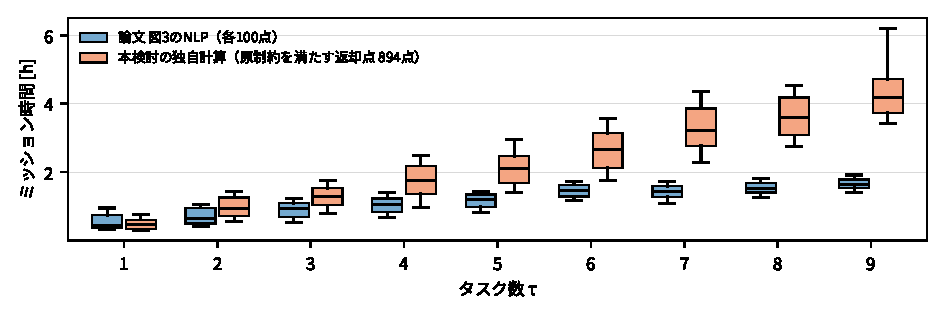
\includegraphics[width=0.95\textwidth]{fig/fig-fig3.pdf}
  \caption{目的値の分布（箱は四分位、ひげは10〜90パーセンタイル）。原論文の値は図3のベクタ図の描画データから読み取った。原論文と独自計算の問題例は対応しない。}
  \label{fig:fig3}
\end{figure}

\answerpart{その他の気づいた点（短く）}
\begin{itemize}
  \item \textbf{$N$ は離散化の細かさだけではない}：$s_k\ge s_{\min}$ から $\sum_ks_k\ge(N-1)s_{\min}$ で、$N$ を増やすと最低時間が増え、実行可能性まで変わりうる。$N$ の影響を確認せずに解法差だけの比較とは読めない。
  \item \textbf{電池写像の区間分割への整合性}：電池残量だけを状態とする時間一様なモデルでは、分割しても結果が変わらない $f(f(e,t_1),t_2)=f(e,t_1+t_2)$ が要る。例えば $f_d(e,t)=e\exp(-at^2)$ は (5) を満たすが、総時間 $T$ を $n$ 等分すると残量が $e\exp(-aT^2/n)$ に変わる。数値例のCC--CVと一定放電はこの整合性を満たす。
\end{itemize}

\FloatBarrier
%======================================================================
\section{問3：問題点1（車両の再訪）の改善案}

\answerpart{改善案}
\begin{table}[H]
  \centering
  \caption{車両の移動を保証するための改善案}
  \label{tab:options}
  \begin{tabular}{p{0.19\textwidth}p{0.4\textwidth}p{0.31\textwidth}}
    \toprule
    案 & 変更と長所 & 負担・限界 \\
    \midrule
    (a) 運用を限定する & 各領域に待機車両を複数置くなど、サービスを外部で保証する。元のモデルをそのまま使える & 必要台数と配置の根拠が別に要る。1台運用の計画にはならない \\
    (b) 再訪間の制約を足す & 充放電と領域の割当を固定し、(R) を加えて再最適化する。車両の変数が要らない & 割当を変えられない。割当自体が実行不能なら直せない \\
    (c) 車両の位置を同時に計画する & 全時点の車両位置を変数にし、充電時にUAVと一致させる。割当も探索できる & 変数・制約が増える。元の非凸性や近似の問題は残る \\
    (d) 事後に検査して直す & 求解後に (R) を検査し、待ち時間や充電を足す。既存の解法に後付けできる & 待つだけでは電池が持たない場合がある（問題点1の10 kmの例） \\
    \bottomrule
  \end{tabular}
\end{table}

\answerpart{検討の過程}
\begin{enumerate}
  \item (24) が一つの区間しか見ていないことに気づき、同じ車両が前の充電の終点から次の始点へ移動する条件として (R) を導いた。原論文の図1の解は (R) を満たすことを確かめ、例の誤りではなくモデルの保証の欠如だと整理した。
  \item 最初は (d) の「足りない時間だけ待つ」を考えたが、充電しない間もUAVは電池を使うので、10 kmの反例では待つだけでは直らないと分かった。充電の場所やモードまで変えられる必要がある。
  \item 独自計算の894点に (R) を当てると590点で不足し、多くは円板内の「跳び」だった。割当固定なら (b) でも車両の移動を保証できる。一方、充電する区間や領域の選択も含めて検討したいので、その拡張を明示しやすい (c) を全体モデルとして選んだ。
  \item 原論文の序論の関連研究整理\cite{yuan}（軌道の混合整数同時最適化、行動順序が既知の場合の二次錐計画、UAVの軌道を先に決める二段階計画）も参考に、(c) を原論文の連続変数の枠組みに入れる方針にした。
\end{enumerate}
以上から、問4では (c) を選ぶ。(b) は (c) で割当を固定した特別な場合として導ける（次節）。

\FloatBarrier
%======================================================================
\section{問4：車両の位置を変数に加えたモデル}

\answerpart{モデルの変更}
各領域 $j$ に車両1台を置き、元の変数 (10) に時点 $k$ の車両位置 $q_{j,k}\in\mathbb R^2$（$j\in[J]$、$k\in[N]$）を加える。目的関数 (1) と制約 (11) はそのままにし、
\begin{equation*}
  \begin{aligned}
  q_{j,k}&\in\mathcal C_j &&(j\in[J],\ k\in[N]),\\
  \norm{q_{j,k+1}-q_{j,k}}&\le v_c\,s_k &&(j\in[J],\ k\in[N-1])
  \end{aligned} \tag{C1}
\end{equation*}
を加える。各 $k\in[N-1]$ の充放電の選言 (12) の後半を、領域条件 $g_j$ の代わりに車両との一致で書き換える。
\begin{equation*}
  \bigvee_{j\in[J]}\left\{c_k=s_k,\ q_{j,k}=r_k,\ q_{j,k+1}=r_{k+1}\right\}\vee\{c_k=0\}. \tag{C2}
\end{equation*}
(C1) と端点の一致から元の (24) は自動的に従う。車両の初期位置 $q_j^0$ が決まっている場合は $q_{j,1}=q_j^0$ を加える（自由にすると、出発前の配置を自由に決められると仮定したことになる）。
円板では (C1) を $\norm{q_{j,k}-o_j}^2\le\rho_j^2$、$\norm{q_{j,k+1}-q_{j,k}}^2\le v_c^2s_k^2$ と2乗して滑らかに書ける（$s_k\ge s_{\min}>0$ なので同値）。
(C2) は原論文と同じく最小値で書き換え、充電の候補値を $\norm{(c_k-s_k,\ q_{j,k}-r_k,\ q_{j,k+1}-r_{k+1},\ \varepsilon)}$ とすればよい。(C1) は選言ではないので、常に課す滑らかな制約になる。

\answerpart{有効と考える理由}
\begin{itemize}
  \item \textbf{区間の間も実行できる}：区間内で $r$ と $q$ を同じ時間比で直線補間すると、円板は凸なので車両は円板内にとどまり、速さは (C1) から $v_c$ 以下である。充電区間では両端が一致するので、区間内の全時刻でUAVと車両が一致する。これにより「跳び」は不可能になる。
  \item \textbf{割当を固定すれば (R) と同値}：領域が凸で、充放電と領域の割当を固定し、初期位置が自由なとき、(C1)、(C2) を満たす $q$ が存在することと、各充電区間で (24)、同じ領域の連続する充電区間 $a<b$ で (R) が成り立つことは同値である。
  必要性は車両が $r_{a+1}$ から $r_b$ まで速さ $v_c$ 以下で動くことから従う。
  十分性は、充電中はUAVと一緒に動き、充電の間は2点を使える時間いっぱいで直線移動し、最初の充電の前と最後の充電の後は止まっている $q$ を作れば示せる。
  初期位置 $q_j^0$ が決まっていれば、最初の充電区間 $a$ について $\norm{r_a-q_j^0}\le v_ct_a$ (C0) も要る。
  よって割当を固定した再最適化では、車両の変数を消して (R)、(C0) だけを加えればよく、これが改善案 (b) である。(R) は距離のノルムを時間の1次式で上から抑える凸制約である。
\end{itemize}

\answerpart{数値での確認}
問題点1の590個から不足距離の分位で6個を選んだ（結果を見る前に規則を決めた）。
充放電・領域・タスクの担当時点を固定し、$q$ありと、$q$を消して(R)のみを課すNLPを、同じ元の返却点からIpopt\cite{ipopt}で解いた。両者の実行可能集合は同じだが、局所解法の挙動は異なりうる。
1500反復・300秒を上限とし、原制約残差$10^{-10}$未満、車両制約の誤差$10^{-9}$ km以下を受理とした。求解時間は1スレッド・直列で各条件1回の予備実行後5回の中央値とし、モデル・ソルバーの生成と後処理を含まない。割当を探索する完全な改善モデルや原論文の解法の検証ではない。
\begin{table}[H]
  \centering
  \caption{固定割当の比較（求解時間はms、問題例は$\tau$/seed）。$q$のτ=9の不受理点の目的値は比較しない。}
  \label{tab:nlp}
  \begin{tabular}{lrrrrr}
    \toprule
    $\tau$/seed & 元の解 [h] & $q$あり [h] & (R)のみ [h] & $q$時間 & (R)時間 \\
    \midrule
    4/4000012 & 2.2923 & 2.2923 & 2.2923 & 13.9 & 134.2 \\
    6/6000032 & 2.4815 & 2.4927 & 2.4927 & 87.8 & 4.2 \\
    8/8000015 & 3.7372 & 3.7516 & 3.7516 & 217.9 & 5.8 \\
    7/7000053 & 3.8816 & 2.8677 & $3.3280^{*}$ & 292.8 & 475.3 \\
    9/9000076 & 4.1605 & 不受理 & 4.1839 & 1012.8 & 413.3 \\
    9/9000001 & 6.2093 & 不受理 & 3.1413 & 1705.9 & 90.4 \\
    \bottomrule
  \end{tabular}
\end{table}
表\ref{tab:nlp}の$^{*}$は反復上限後に区間時間を最大11.95 s延ばして電池を再計算した実行可能点で、収束解ではない。他の(R)5例と$q$4例は成功終了した。同じ目的値に達した$\tau=4,6,8$の3例では、(R)が速いのは2例で、$\tau=4$では逆に約9.7倍遅い（778反復対34反復）。変数削減は一律の高速化を保証しない。
保存済みの車両制約なしの計算と$q$ありの両方が受理された3例の時間差は0〜52 s（0.45\%以下）だったが、少数の局所解の比較であり一般の増加率ではない。図\ref{fig:carrier}の区間21は2.12 km・212 sから30 s・0.09 kmへ縮み、前後の充電や接点の再配置を含め総時間52 sの増加で不足を解消した。保存点の検算と再実行条件は文献\cite{repo}に残した。

\answerpart{有効となる条件・新たに生じる問題・改善できない点}
\begin{itemize}
  \item \textbf{条件}：各領域に車両1台、領域は凸で障害物なし、車両は速度上限だけで表せること。初期位置が決まっているなら (C0) を課す。複数台が来られる運用（改善案 (a)）では、このモデルは厳しすぎる。
  \item \textbf{不収束と実行不能は異なる}：以前$q$ありが不受理だった$\tau=9$の2例でも、UAV位置と割当を変えず、充電を1区間1 hへ延ばす構成で実行可能点を得た（総時間20.9462、20.6399 h）。さらに(R)のみで表の短い解が得られ、その解から$q$ありを始めると両例とも同じ目的値へ27・87反復で成功終了した。固定割当は実行可能であり、不収束は定式化・初期化に依存した。一方、割当も探索する(C2)の平滑化の収束は未検証である。
  \item \textbf{新たに生じる問題}：変数が $2JN$ 個、制約が $O(JN)$ 個増え、探索負担が増す。割当固定なら車両の追加制約自体は凸だが、電池式や割当選択の非凸性は残る。候補値は時間と距離を混ぜるので無次元化が必要であり、有限の$p$では接点の一致も近似になる。最後に原制約と(C1)、(C2)で検査し、必要なら割当固定で修復する必要がある。
  \item \textbf{改善できない点}：道路網・障害物・加速度・車両自身のエネルギー・複数のUAVによる車両の共用は扱えない。ホモトピー法の収束や大域最適性の問題もそのまま残る。
\end{itemize}

\FloatBarrier
{\small\renewcommand{\Needspace}[1]{}%
\begin{thebibliography}{9}
\bibitem{yuan} M.~Yuan, A.~Adane, J.~Humann, and Y.~Yu, ``Nonlinear Trajectory Optimization Models for Uncrewed Aerial Vehicles with Mobile Charging Support,'' arXiv:2609.40201, 2026.
\bibitem{ipopt} A.~W\"achter and L.~T.~Biegler, ``On the Implementation of an Interior-Point Filter Line-Search Algorithm for Large-Scale Nonlinear Programming,'' \textit{Math. Program.}, vol.~106, pp.~25--57, 2006.
\bibitem{repo} 本検討の実装・入力・実験記録，\url{https://github.com/mordent-27/uav}．
\end{thebibliography}}

\end{document}
